% 7-Axis Robot Arm -- joint and axis guide
% compile: xelatex robot-arm-7axis.tex
\documentclass[border=10pt]{standalone}
\usepackage{tikz}
\usetikzlibrary{arrows.meta,bending,calc}

\definecolor{canvasbg}{HTML}{EEF2F7}
\definecolor{cardbg}{HTML}{FFFFFF}
\definecolor{cardline}{HTML}{DCE3EC}
\definecolor{inkdark}{HTML}{1B2430}
\definecolor{inkmid}{HTML}{56637A}
\definecolor{inklite}{HTML}{95A0B4}
\definecolor{armbody}{HTML}{E6EBF2}
\definecolor{armedge}{HTML}{8D9AAF}
\definecolor{armhi}{HTML}{FFFFFF}
\definecolor{axamber}{HTML}{EF9A2E}
\definecolor{axamberlt}{HTML}{FFD199}
\definecolor{axamberdk}{HTML}{9C5A12}
\definecolor{axteal}{HTML}{2E9C93}
\definecolor{axteallt}{HTML}{9BDFD8}
\definecolor{axtealdk}{HTML}{15625C}
\definecolor{gripcol}{HTML}{47536B}
\definecolor{floorcol}{HTML}{C3CEDD}

% ---- a structural link: dark outline, body, specular highlight -------------
\newcommand{\seg}[4]{% start, end, outer width, highlight offset
  \draw[armedge, line cap=round, line width=#3] (#1) -- (#2);
  \draw[armbody, line cap=round, line width=\dimexpr#3-2.6pt\relax] (#1) -- (#2);
  \draw[armhi, line cap=round, line width=\dimexpr#3/4\relax, opacity=0.9,
        shorten >=3pt, shorten <=3pt]
    ($(#1)!#4!90:(#2)$) -- ($(#2)!#4!-90:(#1)$);
}

% ---- a revolute joint drawn as a short cylinder ----------------------------
\newcommand{\jointgen}[6]{% coord, axis angle, radius, main, light, dark
  \begin{scope}[shift={(#1)}, rotate=#2]
    \fill[#6] (-0.24,0) ellipse [x radius=0.13, y radius=#3];
    \fill[#4] (-0.24,-#3) rectangle (0.24,#3);
    \fill[#5, opacity=0.55] (-0.24,{0.32*#3}) rectangle (0.24,#3);
    \fill[#6, opacity=0.30] (-0.24,-#3) rectangle (0.24,{-0.55*#3});
    \draw[#6, line width=0.7pt] (-0.24,#3) -- (0.24,#3);
    \draw[#6, line width=0.7pt] (-0.24,-#3) -- (0.24,-#3);
    \fill[#5] (0.24,0) ellipse [x radius=0.13, y radius=#3];
    \draw[#6, line width=0.8pt] (0.24,0) ellipse [x radius=0.13, y radius=#3];
    \fill[#6, opacity=0.55] (0.24,0) ellipse [x radius=0.05, y radius={0.34*#3}];
  \end{scope}
}
\newcommand{\jointA}[3]{\jointgen{#1}{#2}{#3}{axamber}{axamberlt}{axamberdk}}
\newcommand{\jointB}[3]{\jointgen{#1}{#2}{#3}{axteal}{axteallt}{axtealdk}}

% ---- the rotation axis itself ----------------------------------------------
\newcommand{\axisray}[4]{% coord, angle, half length, colour
  \draw[#4, line width=0.9pt, dash pattern=on 3.4pt off 2.6pt, opacity=0.85]
    ($(#1)+({#2}:{#3})$) -- ($(#1)+({#2+180}:{#3})$);
}

% ---- curved arrow wrapping the axis ----------------------------------------
\newcommand{\spin}[5]{% coord, angle, radius, offset along axis, colour
  \begin{scope}[shift={(#1)}, rotate=#2]
    \draw[#5, line width=1.15pt, -{Stealth[length=4.8pt,width=3.8pt,bend]}]
      ({#4},{-1.32*#3})
      arc[start angle=-90, end angle=158, x radius=0.19, y radius={1.32*#3}];
  \end{scope}
}

\begin{document}
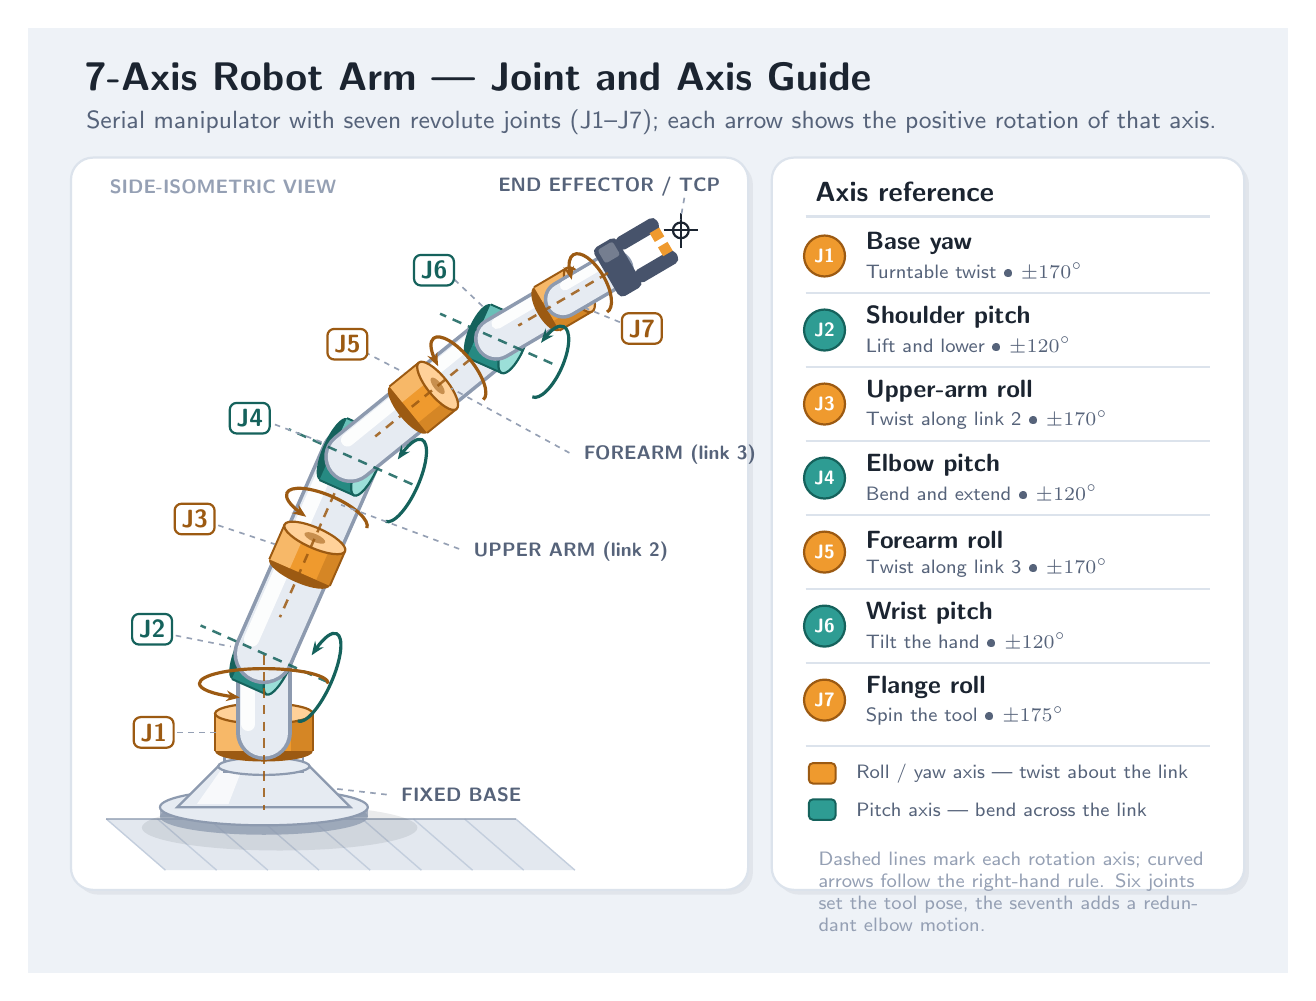
\begin{tikzpicture}[font=\sffamily, x=1cm, y=1cm]

% ============================ canvas & cards ===============================
\fill[canvasbg] (0,0) rectangle (16,12);

\fill[inkdark, opacity=0.06, rounded corners=8pt] (0.61,0.99) rectangle (9.21,10.29);
\fill[cardbg, draw=cardline, line width=0.8pt, rounded corners=8pt]
      (0.55,1.05) rectangle (9.15,10.35);
\fill[inkdark, opacity=0.06, rounded corners=8pt] (9.51,0.99) rectangle (15.51,10.29);
\fill[cardbg, draw=cardline, line width=0.8pt, rounded corners=8pt]
      (9.45,1.05) rectangle (15.45,10.35);

\node[anchor=west, font=\sffamily\bfseries\Large, text=inkdark]
      at (0.60,11.38) {7-Axis Robot Arm \textemdash{} Joint and Axis Guide};
\node[anchor=west, font=\sffamily\small, text=inkmid] at (0.62,10.80)
      {Serial manipulator with seven revolute joints (J1--J7); each arrow shows the positive rotation of that axis.};

\node[anchor=west, font=\sffamily\bfseries\scriptsize, text=inklite]
      at (0.92,9.98) {SIDE-ISOMETRIC VIEW};

% ============================== joint frame ================================
\coordinate (J1) at (3.00,3.05);
\coordinate (J2) at (3.00,4.05);
\coordinate (J3) at (3.55,5.30);
\coordinate (J4) at (4.10,6.55);
\coordinate (J5) at (5.02,7.30);
\coordinate (J6) at (5.95,8.05);
\coordinate (J7) at (6.80,8.55);
\coordinate (FL) at (7.45,8.93);

% ================================ floor ====================================
\fill[floorcol, opacity=0.45] (1.00,1.95) -- (6.20,1.95) -- (6.95,1.30) -- (1.75,1.30) -- cycle;
\foreach \k in {0,...,8}{%
  \draw[floorcol, line width=0.5pt] ({1.00+\k*0.65},1.95) -- ({1.75+\k*0.65},1.30);}
\draw[armedge, line width=0.7pt, opacity=0.7] (1.00,1.95) -- (6.20,1.95);
\fill[inkdark, opacity=0.09] (3.20,1.84) ellipse [x radius=1.75, y radius=0.29];

% ============================== pedestal ===================================
\fill[armedge, opacity=0.75] (3.00,1.98) ellipse [x radius=1.32, y radius=0.23];
\fill[armedge, opacity=0.75] (1.68,1.98) rectangle (4.32,2.10);
\fill[armbody, draw=armedge, line width=0.8pt] (3.00,2.10) ellipse [x radius=1.32, y radius=0.23];
\fill[armbody, draw=armedge, line width=0.8pt]
      (1.90,2.10) -- (4.10,2.10) -- (3.58,2.62) -- (2.42,2.62) -- cycle;
\fill[armhi, opacity=0.75] (2.15,2.14) -- (2.55,2.14) -- (2.72,2.58) -- (2.46,2.58) -- cycle;
\fill[armbody, draw=armedge, line width=0.8pt] (2.50,2.55) rectangle (3.50,2.98);
\fill[armhi, opacity=0.8] (2.62,2.58) rectangle (2.80,2.96);
\fill[armbody, draw=armedge, line width=0.8pt] (3.00,2.62) ellipse [x radius=0.58, y radius=0.11];

% ========================= links and joints ================================
\jointA{J1}{90}{0.62}
\seg{J1}{J2}{20pt}{5.6pt}
\jointB{J2}{-24}{0.46}
\seg{J2}{J4}{22pt}{6.2pt}
\jointA{J3}{66.25}{0.42}
\jointB{J4}{-24}{0.43}
\seg{J4}{J6}{19pt}{5.4pt}
\jointA{J5}{39.05}{0.38}
\jointB{J6}{-24}{0.37}
\seg{J6}{J7}{16pt}{4.6pt}
\jointA{J7}{30.4}{0.32}
\seg{J7}{FL}{14pt}{4.0pt}

% ============================ end effector =================================
\begin{scope}[shift={(FL)}, rotate=30.4]
  \fill[gripcol, rounded corners=2pt] (-0.12,-0.36) rectangle (0.22,0.36);
  \fill[armhi, opacity=0.25, rounded corners=1pt] (-0.06,0.12) rectangle (0.16,0.32);
  \fill[gripcol, rounded corners=2pt] (0.18,0.15) rectangle (0.78,0.33);
  \fill[gripcol, rounded corners=2pt] (0.18,-0.33) rectangle (0.78,-0.15);
  \fill[axamber] (0.62,0.04) rectangle (0.76,0.17);
  \fill[axamber] (0.62,-0.17) rectangle (0.76,-0.04);
  \coordinate (TCP) at (0.98,0.00);
\end{scope}
\draw[inkdark, line width=0.8pt] (TCP) circle [radius=0.10];
\draw[inkdark, line width=0.8pt] ($(TCP)+(-0.22,0)$) -- ($(TCP)+(0.22,0)$);
\draw[inkdark, line width=0.8pt] ($(TCP)+(0,-0.22)$) -- ($(TCP)+(0,0.22)$);

% ======================= axes and rotation arrows ==========================
\axisray{J1}{90}{0.98}{axamberdk}
\axisray{J2}{-24}{0.88}{axtealdk}
\axisray{J3}{66.25}{0.86}{axamberdk}
\axisray{J4}{-24}{0.86}{axtealdk}
\axisray{J5}{39.05}{0.78}{axamberdk}
\axisray{J6}{-24}{0.78}{axtealdk}
\axisray{J7}{30.4}{0.66}{axamberdk}

\spin{J1}{90}{0.62}{0.62}{axamberdk}
\spin{J2}{-24}{0.46}{0.74}{axtealdk}
\spin{J3}{66.25}{0.42}{0.62}{axamberdk}
\spin{J4}{-24}{0.43}{0.74}{axtealdk}
\spin{J5}{39.05}{0.38}{0.58}{axamberdk}
\spin{J6}{-24}{0.37}{0.72}{axtealdk}
\spin{J7}{30.4}{0.32}{0.40}{axamberdk}

% ============================== callouts ===================================
\begin{scope}[inklite, line width=0.6pt, dash pattern=on 2pt off 2pt]
  \draw (1.90,3.05) -- (2.40,3.05);
  \draw (1.88,4.28) -- (2.58,4.14);
  \draw (2.42,5.68) -- (3.14,5.44);
  \draw (3.14,6.96) -- (3.78,6.72);
  \draw (4.28,7.88) -- (4.78,7.62);
  \draw (5.42,8.80) -- (5.80,8.44);
  \draw (7.52,8.26) -- (7.08,8.44);
  \draw (4.56,2.26) -- (3.86,2.34);
  \draw (5.48,5.38) -- (3.98,5.94);
  \draw (6.88,6.60) -- (5.38,7.42);
  \draw (8.34,9.84) -- (8.29,9.56);
\end{scope}

\tikzset{
  jlabA/.style={fill=cardbg, draw=axamberdk, line width=0.8pt, rounded corners=2.5pt,
                inner sep=2.4pt, text=axamberdk, font=\sffamily\bfseries\small},
  jlabB/.style={fill=cardbg, draw=axtealdk, line width=0.8pt, rounded corners=2.5pt,
                inner sep=2.4pt, text=axtealdk, font=\sffamily\bfseries\small},
  partlab/.style={font=\sffamily\bfseries\scriptsize, text=inkmid},
}
\node[jlabA] at (1.60,3.05) {J1};
\node[jlabB] at (1.58,4.36) {J2};
\node[jlabA] at (2.12,5.76) {J3};
\node[jlabB] at (2.82,7.04) {J4};
\node[jlabA] at (4.06,7.98) {J5};
\node[jlabB] at (5.16,8.92) {J6};
\node[jlabA] at (7.80,8.18) {J7};

\node[partlab, anchor=west] at (4.62,2.26) {FIXED BASE};
\node[partlab, anchor=west] at (5.54,5.34) {UPPER ARM (link 2)};
\node[partlab, anchor=west] at (6.94,6.58) {FOREARM (link 3)};
\node[partlab, anchor=east] at (8.92,9.98) {END EFFECTOR / TCP};

% =============================== panel =====================================
\node[anchor=west, font=\sffamily\bfseries, text=inkdark] at (9.88,9.92) {Axis reference};
\draw[cardline, line width=0.9pt] (9.88,9.60) -- (15.02,9.60);

\foreach [count=\i] \tg/\ca/\cb/\ttl/\dsc in {%
  J1/axamber/axamberdk/Base yaw/{Turntable twist \textbullet{} $\pm170^{\circ}$},
  J2/axteal/axtealdk/Shoulder pitch/{Lift and lower \textbullet{} $\pm120^{\circ}$},
  J3/axamber/axamberdk/Upper-arm roll/{Twist along link 2 \textbullet{} $\pm170^{\circ}$},
  J4/axteal/axtealdk/Elbow pitch/{Bend and extend \textbullet{} $\pm120^{\circ}$},
  J5/axamber/axamberdk/Forearm roll/{Twist along link 3 \textbullet{} $\pm170^{\circ}$},
  J6/axteal/axtealdk/Wrist pitch/{Tilt the hand \textbullet{} $\pm120^{\circ}$},
  J7/axamber/axamberdk/Flange roll/{Spin the tool \textbullet{} $\pm175^{\circ}$}%
}{%
  \pgfmathsetmacro{\y}{9.10-(\i-1)*0.94}
  \node[circle, fill=\ca, draw=\cb, line width=0.8pt, minimum size=0.52cm,
        inner sep=0pt, text=white, font=\sffamily\bfseries\scriptsize] at (10.12,\y) {\tg};
  \node[anchor=west, font=\sffamily\bfseries\small, text=inkdark] at (10.52,{\y+0.16}) {\ttl};
  \node[anchor=west, font=\sffamily\scriptsize, text=inkmid] at (10.52,{\y-0.20}) {\dsc};
  \ifnum\i<7\relax
    \draw[cardline, line width=0.5pt] (9.88,{\y-0.47}) -- (15.02,{\y-0.47});
  \fi
}

\draw[cardline, line width=0.9pt] (9.88,2.88) -- (15.02,2.88);

\fill[axamber, draw=axamberdk, line width=0.7pt, rounded corners=1.5pt]
      (9.92,2.40) rectangle (10.26,2.66);
\node[anchor=west, font=\sffamily\scriptsize, text=inkmid] at (10.40,2.53)
      {Roll / yaw axis \textemdash{} twist about the link};
\fill[axteal, draw=axtealdk, line width=0.7pt, rounded corners=1.5pt]
      (9.92,1.94) rectangle (10.26,2.20);
\node[anchor=west, font=\sffamily\scriptsize, text=inkmid] at (10.40,2.07)
      {Pitch axis \textemdash{} bend across the link};

\node[anchor=north west, font=\sffamily\scriptsize, text=inklite, text width=5.05cm,
      align=left] at (9.92,1.66)
      {Dashed lines mark each rotation axis; curved arrows follow the right-hand rule.
       Six joints set the tool pose, the seventh adds a redundant elbow motion.};

\end{tikzpicture}
\end{document}
